\tableofcontents
\newpage
\section{Scelta Capitolato}
\subsection{Dall'analisi alla scelta}
\paragraph{}
A seguito degli incontri esplorativi con i proponenti e annessi studi interni
al gruppo, quest'ultimo ha deciso di candidarsi per il progetto Smart4Energy,
proposto dall'azienda \copyright Socomec.\\
Successivamente ad un approfondimento individuale prima e con i proponenti dopo,
il Team ha esposto le proprie preferenze stilando una classifica a punteggio per
decretarne, infine, una generale che riassumeva le volontà generali del gruppo.\\
Per sfruttare la maggiore democraticità possibile, ogni membro del gruppo ha
espresso le proprie preferenze in una classifica di 6 posizioni, abbinando ad
ogni posizione un punteggio che parte da 6 e decresce di 1 ad ogni posizione.
La classifica finale dei punteggi e, dunque, delle preferenze è data dalla somma
dei punteggi che ogni capitolato ha ottenuto dalle singole votazioni.\\
In un primo momento la prima classifica generale, basata solamente sui punteggi
delle singole preferenze, risultava la seguente:\\

\begin{center}
    \begin{tabular}{|c|l|l|}
    \hline
        Posizione & Capitolato & Proponente\\
        \hline
        1 & Social Guida Michelin & ZERO12 \\
        2 & Bot4Me & Imola Informatica \\
        3 & BlockChange & SyncLab \\
        4 & Smart4Energy & Socomec \\
        5 & CC4D & SanMarco informatica \\
        6 & Login Warrior & Zucchetti SPA \\
        \hline
    \end{tabular}
\end{center}
\paragraph{}
Preso atto della prima graduatoria, il gruppo ha discusso uno ad uno i capitolati,
proponendo una analisi dei Pro e dei Contro di  ciascun progetto e relativo proponente,
sollevando quindi le possibili criticità.\\
Ad una più attenta analisi quindi, la classifica si è ridisposta come segue:\\
\begin{center}
    \begin{tabular}{|c|l|l|}
    \hline
        Posizione & Capitolato & Proponente\\
        \hline
        1 & Social Guida Michelin & ZERO12 \\
        2 & Smart4Energy & Socomec \\
        3 & Bot4Me & Imola informatica \\
        4 & BlockChange & SyncLab \\
        5 & CC4D & SanMarco informatica \\
        6 & Login Warrior & Zucchetti SPA \\
        \hline
    \end{tabular}
\end{center}
\paragraph{}
Il team ha quindi deciso di effettuare degli incontri esplorativi con i primi
tre proponenti classificati, al termine dei quali si è giunti alla conclusione
definitiva di scegliere il capitolato Smart4Energy dell'azienda
\copyright Socomec.\\
\newpage
\subsection{Motivazioni della scelta di Smart4Energy}
\paragraph{}
La scelta del capitolato Smart4Energy proviene, di conseguenza, da un interesse
incrementatosi dopo il colloquio avuto con il proponente. L'affinità con l'ambiente
tecnico dell'azienda rendeva il team parecchio restio all'approccio verso questa
scelta, ma la discussione ha evidenziato come i punti di contatto tra le nostre
necessità di lavoro e di apprendimento come team e le aspettative aziendali fossero
molti più di quelli attesi. \\
Da questo quadro filtra principalmente il desiderio dell'azienda di unire la propria
esperienza tecnica nel settore con il guizzo creativo che il nostro gruppo si
propone di offrire; guidandoci attivamente nel percorso mediante contatto costante
e linee di comunicazione efficienti. \\
L 'ampia libertà nell'uso delle tecnologie, l'esposizione chiara degli obiettivi e
l'utilità accademica e pratica del prodotto finale sono state una grande attrattiva
per il team, che ha convogliato il comune interesse per il mondo IOT verso questo
capitolato e ci ha permesso di prendere distanza dal preconcetto creatosi in principio. \\
La proposta dell'azienda rappresenta per noi, dunque, il giusto compromesso di fattibilità
ed il punto di equilibrio tra le estreme libertà progettuali e le rigide direttive aziendali di cui il gruppo necessita.
\subsection{Capitolati scartati}
\paragraph{}
Di seguito si hanno le conclusioni tratte dall'analisi individuale dei singoli progetti scartati:
\begin{enumerate}
    \item \textbf{Social Guida Michelin} \\
      Benché risulti una proposta stimolante per tutto il gruppo, il capitolato C4 prevede un grado di libertà
      progettuale molto elevato che rischia di sfuggire dalla nostra portata. Le tecnologie utilizzabili sono
      le più vaste e, in particolare, la necessaria conoscenza di AWS dilaterebbe a dismisura i tempi di
      apprendimento personale.\\
      In aggiunta, la tecnologia dei crawler risulta un nodo critico;  data soprattutto la poca prevedibilità
      di reazione delle piattaforme in cui vengono impiegati e l'insorgenza di intoppi indipendenti dalle attività
      di progettazione e realizzazione del gruppo.\\
      Il team ha deciso pertanto, a seguito dell'incontro con il proponente, di scartare il capitolato.
    \item \textbf{Bot4Me} \\ 
      L'estrema libertà dataci dall'azienda risulta un'arma a doppio taglio per la scelta di questo capitolato.
      Dalla presentazione in aula ne emerge un'idea ben precisa, ma con una più fumosa rappresentazione sul piano
      pratico e progettuale.\\ Il grande range di features richieste per questo progetto rende l'attività molto
      ampia e pericolosamente frammentaria. Considerando anche la difficile posizione topografica dell'azienda,
      riteniamo che la distanza sia un ulteriore deterrente che renderebbe difficili le collaborazioni durante
      il progetto o future.\\ Il fatto che sia stato difficile contattare l'azienda ha influito sulla scelta finale.
    \item \textbf{BlockChange} \\ 
      L'utilizzo di tecnologie estremamente attuali è il punto forte di questo capitolato, che permette apparente
      dinamicità nelle scelte progettuali. Lavorare con le crypto-valute è risultato attraente per molti membri
      del gruppo, ma all'unanimità concordiamo sulla grande dispersività che un progetto di questo calibro può
      comportare. \\
      Addentrarci in un tale terreno inesplorato risulterebbe dannoso sia per la produttività del gruppo, sia per
      la mancata soddisfazione delle aspettative dell'azienda.
    \newpage
    \item \textbf{CC4D} \\
      Il capitolato C3 prevede una scelta molto ristretta e vincolata di tecnologie e scelte progettuali che mal
      si sposano con gli interessi e le esigenze del nostro gruppo.\\
      Nonostante venga apprezzata la rigorosità nella descrizione dei risultati attesi, la convergenza verso le
      macchine produttive risulta limitante sia per la realizzazione di questo progetto sia per prospettive
      future di utilizzo delle conoscenze apprese.
    \item \textbf{Login Warrior} \\
      Nonostante il gruppo ritenga valida la fattibilità del progetto, le attività principalmente richieste,
      ovvero la raccolta e l' analisi dei dati, combinate con l'inserimento in una realtà estremamente vasta come
      quella dell'azienda in questione,  non soddisfano l'interesse e le nostre aspettative di lavoro.\\
      Il primo vincolo preclude la sperimentazione con tecnologie e attività che divergano dagli obiettivi
      descritti, mentre il secondo renderebbe sicuramente il supporto e l'integrazione nell'ambiente lavorativo
      marginale.
\end{enumerate}

\newpage

\section{Impegni}
\subsection{Scadenza ultima consegna}
\paragraph{}
A monte degli incontri con l’azienda proponente del capitolato d'interesse
e delle precedenti discussioni del team riguardo le tempistiche di realizzazione
del progetto, il gruppo Carbon7team definisce la data di scadenza ultima di
consegna del lavoro al \textbf{10 aprile 2022}.\\Carbon7team si impegna a rispettare tale
scadenza e ritiene fattibile poter svolgere l’incarico entro la data
comunicata.
\subsection{Totale ore produttive}
\paragraph{}
Considerando l’intervallo di tempo dall’inizio della realizzazione del
progetto, ovvero dal momento dell’aggiudicazione dell’appalto, fino alla
data di scadenza ultima di consegna indicata, ogni membro del gruppo si
è reso disponibile e si impegna a svolgere \textbf{100 ore produttive di lavoro}
dedicate al progetto. Considerando la numerosità del team, ne consegue un
\textbf{totale di 700 ore produttive di lavoro} per il completamento delle attività.
Carbon7team ritiene che questa cifra sia sufficiente per portare a termine
l’incarico.
\subsection{Preventivo dei costi}
\paragraph{}
Le ore produttive di lavoro totali sono state distribuite tra i vari ruoli
in modo che tutti abbiano sufficienti ore per assicurare la fattibilità del
progetto. Sommando le ore produttive di lavoro totali assegnate ad ogni ruolo
e pesandole con il relativo costo orario, si ottiene il costo totale di progetto
di \textbf{€14.035}, rispettando la soglia minima fissata.\\Il team si impegna a
distribuire i ruoli ai vari membri garantendo assenza di conflitti di interesse
e rotazione; in modo che ogni elemento del gruppo ricopra ogni ruolo almeno una
volta e per un tempo proporzionalmente congruo.\\La seguente tabella mostra il
preventivo dei costi sulla base del totale ore/ruoli.\\\\
\begin{center}
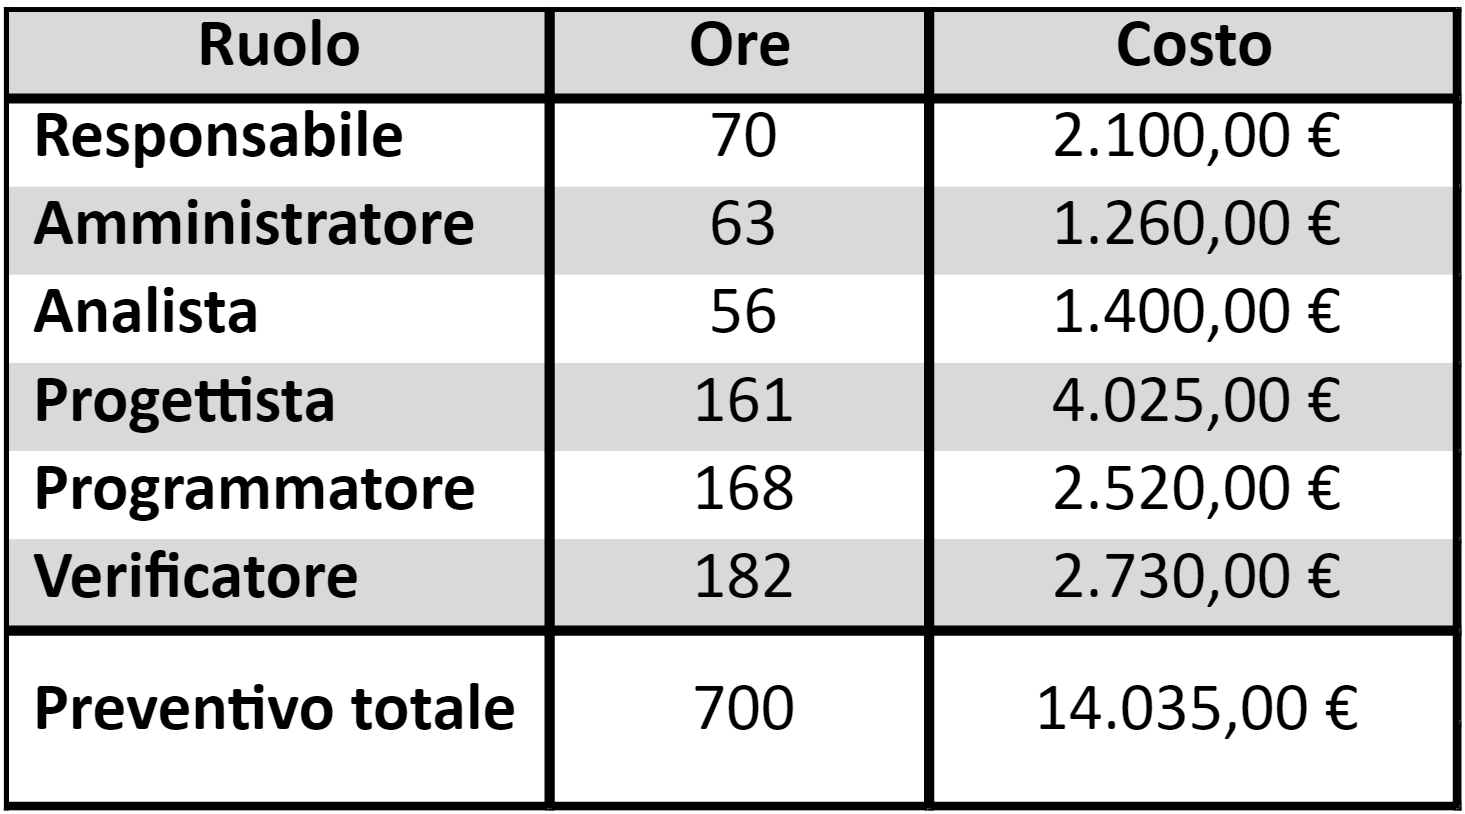
\includegraphics[scale=0.3]{res/images/tabella_costi.png}
\end{center}
\newpage
\section{Resoconto degli incontri esplorativi con i proponenti}
\paragraph{}
In allegato al documento di candidatura, si trovano i verbali dei due incontri
esplorativi avuti con i proponenti \copyright ZERO12 e \copyright Socomec,
nonché quello per l'incontro di conferma con quest'ultima azienda:
\begin{itemize}
  \item Primo incontro con Socomec
  \item Primo incontro con ZERO12
  \item Secondo incontro con Socomec - Conferma
\end{itemize}
Link: \textcolor{blue}{\underline{\url{https://github.com/Carbon7team/Docs/Interni/Verbali}}}